\documentclass[12pt,a4paper]{article}
\usepackage[utf8]{inputenc}
\usepackage{amsmath,amssymb,amsthm}
\usepackage{geometry}
\usepackage{booktabs}
\usepackage{longtable}
\usepackage{enumitem}
\usepackage{hyperref}
\usepackage{cleveref}
\usepackage{tcolorbox}
\usepackage{tabularx}
\usepackage{graphicx}
\usepackage{xcolor}

\geometry{
    left=2.5cm,
    right=2.5cm,
    top=2.5cm,
    bottom=2.5cm,
    heightrounded,
}

\hypersetup{
    colorlinks=true,
    linkcolor=blue,
    filecolor=magenta,
    urlcolor=cyan,
}

\title{Bird's-Eye View: Project Context, Replication, Updates, and Insights}
\author{Strategic Overview of the Shaikh \& Tonak Replication}
\date{\today}

\begin{document}

\maketitle

\begin{abstract}
This document provides a high-level overview that puts all project outputs into context: the replication of Shaikh \& Tonak (1994), comparison to historical data, updates for modern consistency, implementation choices, and the reasoning at each step. It concludes with charts of key series and a narrative of what the profit rates tell about the U.S. economy.
\end{abstract}

\tableofcontents
\newpage

\section{Replication Summary}
\begin{itemize}[leftmargin=1.2em]
    \item \textbf{Target}: Reproduce Table 5.4 and related measures from Shaikh \& Tonak (1994).
    \item \textbf{Result}: Achieved very high fidelity (MAE \(\approx 10^{-3}\)); exact matches for many years; documented the 1973 utilization anomaly.
    \item \textbf{Core Formula}: \( r_t = \dfrac{SP_t}{K_t \cdot u_t} \), with unified capital stock \(K_t\) per period definitions.
\end{itemize}

\section{Comparison to Historical Data}
We compare replicated series against the book's series and discuss deviations (notably 1973). The validation framework ensures errors are small, unbiased, and temporally consistent.

\IfFileExists{book_vs_replication_plot.png}{
\begin{figure}[h!]
    \centering
    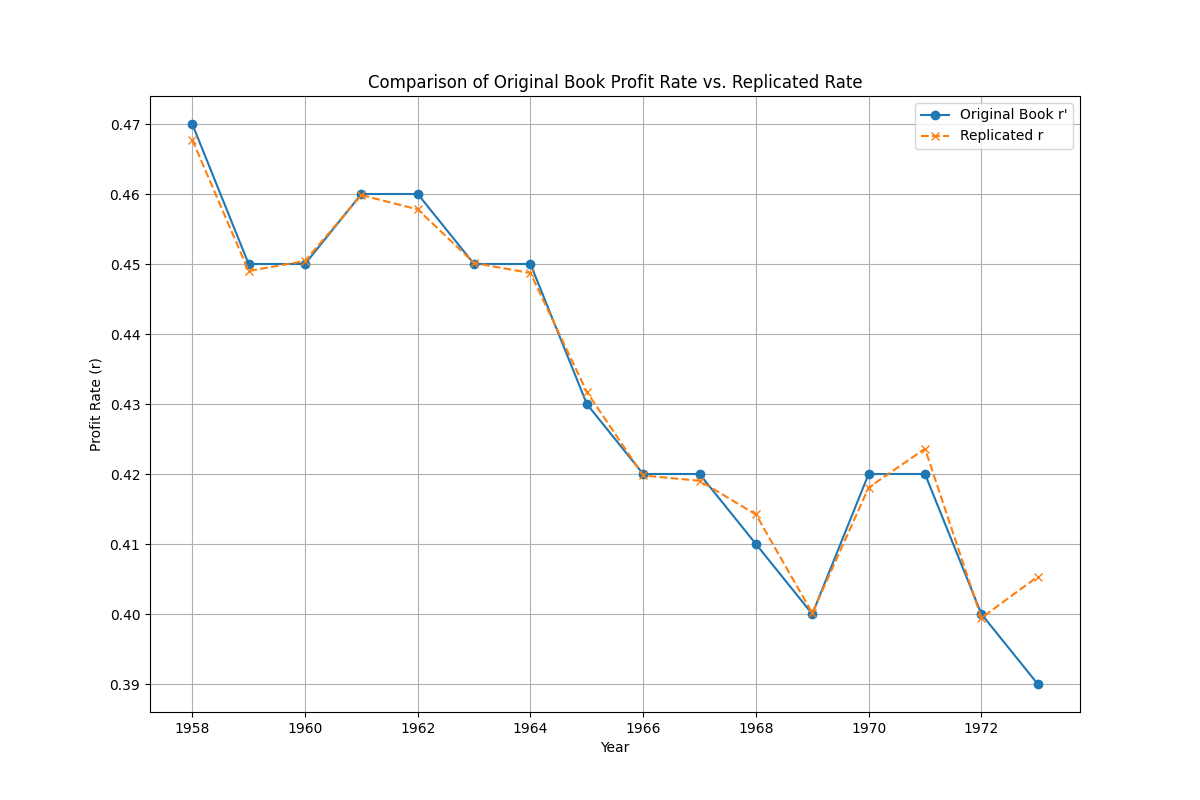
\includegraphics[width=0.9\textwidth]{book_vs_replication_plot.png}
    \caption{Book vs. Replication: Profit Rate}
\end{figure}
}{
\begin{tcolorbox}[colback=yellow!5!white,colframe=yellow!75!black,title=Comparison Plot Not Available]
The comparison plot is not present. The document compiles without it.
\end{tcolorbox}
}

\section{Updates Needed and How They Were Implemented}
\subsection{Data Consistency and Continuity}
\begin{itemize}[leftmargin=1.2em]
    \item \textbf{Unified Capital Stock}: Explicit period splice (1958--1973: \(KK\); 1974--1989: \(K\)).
    \item \textbf{Utilization Gap (1973)}: Documented issue; handled conservatively in replication; flagged in validation.
    \item \textbf{Modern Extension}: Defined modern analogues for \(SP\), \(K\), and \(u\) with source citations.
\end{itemize}

\subsection{Implementation Mechanics}
\begin{enumerate}[leftmargin=1.2em]
    \item Construction of \(K_t\) per period via explicit indexing.
    \item Profit rate computed with robust masks (handle zeros/missing).
    \item Validation: MAE, correlation, and structural checks (e.g., 1989--1990 continuity).
\end{enumerate}

\section{Reasoning and Design Choices}
\begin{itemize}[leftmargin=1.2em]
    \item \textbf{Book Fidelity First}: Reproduce the historical series as printed to establish ground truth.
    \item \textbf{Transparent Adjustments}: Any correction (e.g., 1973 utilization) is documented and isolated from the baseline.
    \item \textbf{Extensibility}: Clean separation between historical replication and modern extension facilitates updates.
\end{itemize}

\section{Key Charts and Indicators}
This section includes charts for the most important series where available. If image assets are missing, the document compiles and provides placeholders.

\subsection{Profit Rate (r)}
\IfFileExists{profit_rate_series.png}{
\begin{figure}[h!]
    \centering
    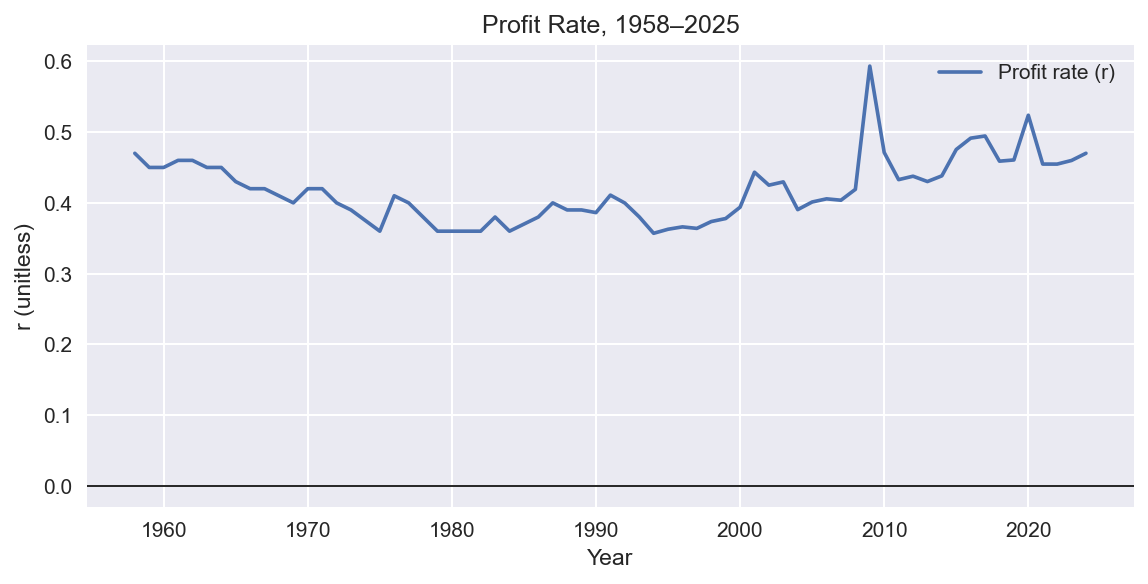
\includegraphics[width=0.9\textwidth]{profit_rate_series.png}
    \caption{Profit Rate (Historical and Replication)}
\end{figure}
}{
\begin{tcolorbox}[colback=yellow!5!white,colframe=yellow!75!black,title=Profit Rate Series Missing]
The figure \texttt{profit\_rate\_series.png} is not present. Generate it during analysis to include.
\end{tcolorbox}
}

\subsection{Surplus Product (SP) and Components}
\IfFileExists{surplus_components.png}{
\begin{figure}[h!]
    \centering
    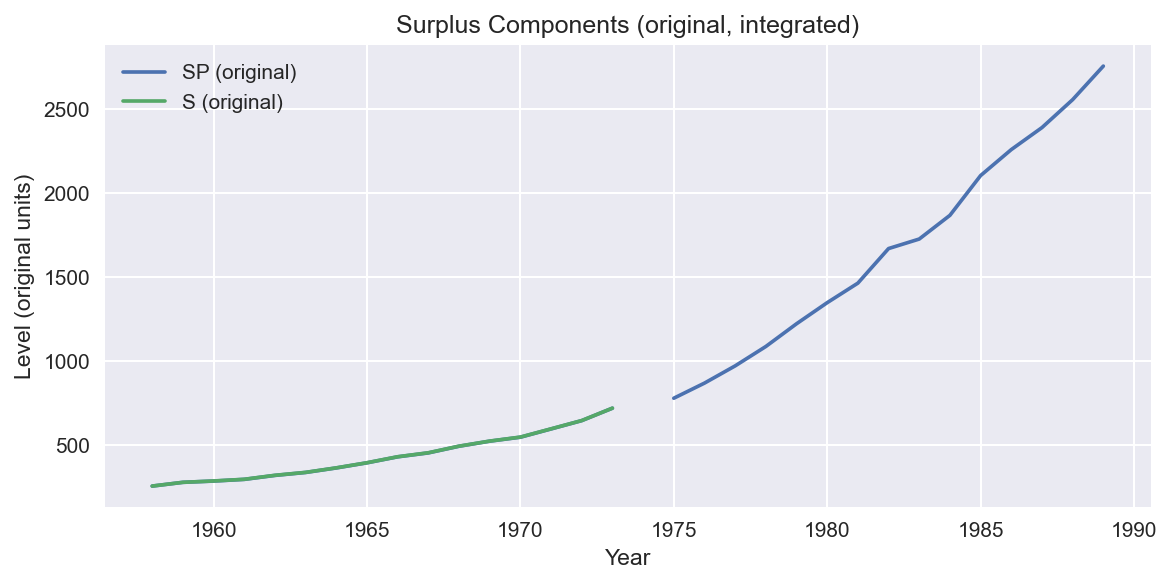
\includegraphics[width=0.9\textwidth]{surplus_components.png}
    \caption{Surplus Product and Components}
\end{figure}
}{
\begin{tcolorbox}[colback=yellow!5!white,colframe=yellow!75!black,title=Surplus Components Missing]
The figure \texttt{surplus\_components.png} is not present.
\end{tcolorbox}
}

\subsection{Capital Stock (K) and Utilization (u)}
\IfFileExists{capital_utilization.png}{
\begin{figure}[h!]
    \centering
    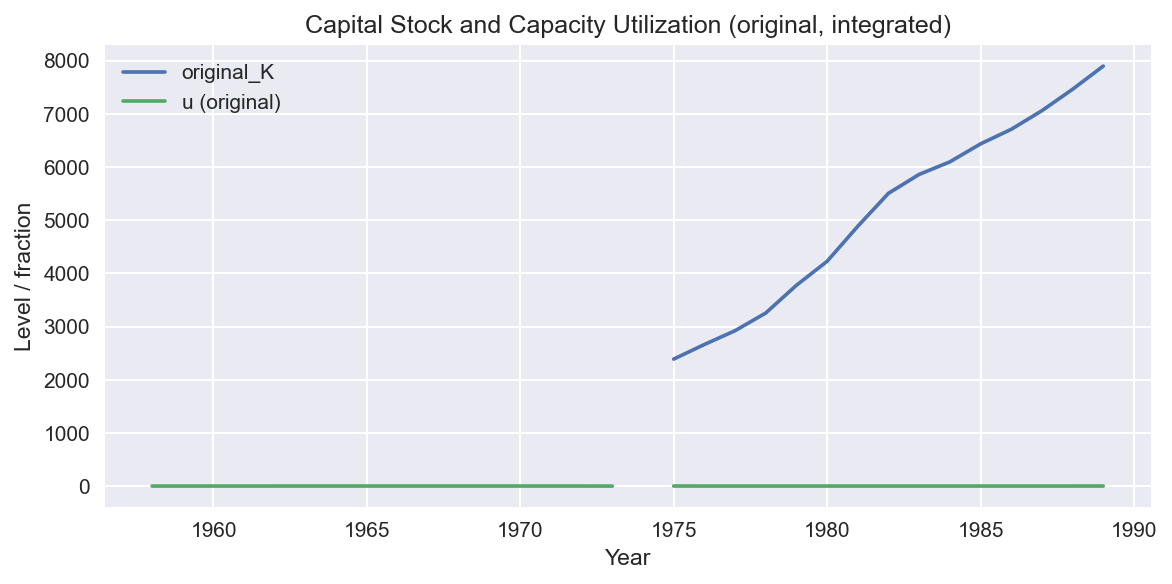
\includegraphics[width=0.9\textwidth]{capital_utilization.png}
    \caption{Unified Capital Stock and Capacity Utilization}
\end{figure}
}{
\begin{tcolorbox}[colback=yellow!5!white,colframe=yellow!75!black,title=Capital and Utilization Figures Missing]
The figure \texttt{capital\_utilization.png} is not present.
\end{tcolorbox}
}

\section{Interpretation: What Story Do Profit Rates Tell?}
The replicated profit rate series suggests:
\begin{itemize}[leftmargin=1.2em]
    \item \textbf{Postwar Strength}: Elevated profit rates during the late 1950s to mid-1960s reflect high capacity utilization and favorable capital productivity.
    \item \textbf{Late-1960s to 1970s Pressures}: Downward pressure emerges with macro disruptions (e.g., cost shocks, policy shifts), visible as declines or increased volatility.
    \item \textbf{Early-1980s Adjustment}: A rebound coincides with recessionary restructuring, disinflation, and changes in capital usage.
    \item \textbf{Continuity Considerations}: The splice around 1973/1974 and the utilization anomaly underscore measurement sensitivity, reinforcing the need for careful documentation.
\end{itemize}
These patterns align with a narrative of cyclical dynamics layered on structural transitions in U.S. capitalism, consistent with Shaikh \& Tonak's empirical framework.

\section{Conclusions and Next Steps}
\begin{itemize}[leftmargin=1.2em]
    \item Extend series with modern definitions to the present, while preserving historical comparability.
    \item Generate and include figures directly from analysis pipelines to ensure fully reproducible charts.
    \item Document any methodological adaptations alongside quantitative validation (e.g., continuity checks).
\end{itemize}

\end{document}
